\graphicspath{ {images/} }

\titledquestion{Attention exploration}[20]
\label{sec:analysis}

Multi-head self-attention is the core modeling component of Transformers.
In this question, we'll get some practice working with the self-attention equations, and motivate why multi-headed self-attention can be preferable to single-headed self-attention.

Recall that attention can be viewed as an operation on a \textit{query} vector $q\in\mathbb{R}^d$, a set of \textit{value} vectors $\{v_1,\dots,v_n\}, v_i\in\mathbb{R}^d$, and a set of \textit{key} vectors $\{k_1,\dots,k_n\}, k_i \in \mathbb{R}^d$, specified as follows:
\begin{align}
&c = \sum_{i=1}^{n} v_i \alpha_i \\
&\alpha_i = \frac{\exp(k_i^\top q)}{\sum_{j=1}^{n} \exp(k_j^\top q)}
\end{align} 
with $alpha = \{\alpha_1, \ldots, \alpha_n\}$ termed the ``attention weights''. 
Observe that the output $c\in\mathbb{R}^d$ is an average over the value vectors weighted with respect to $\alpha$.

\begin{parts}

\part[5] \textbf{Copying in attention.} One advantage of attention is that it's particularly easy to ``copy'' a value vector to the output $c$. In this problem, we'll motivate why this is the case.

\begin{subparts}
    \subpart[1] \textbf{Explain} why $\alpha$ can be interpreted as a categorical probability distribution. 
    
    \ifans{
        \begin{enumerate}
            \item The attention weights are normalized through a \textbf{softmax} function, meaning that they can take on any value between 0 and 1 and their sum equals 1.
            \item Attention weights are often used to determine the \textbf{relevance} or \textbf{similarity} of different elements within a sequence. Each element's weight represents the probability of its relevance or similarity. 
            \item Interpreting attention weights as a categorical probability distribution is useful because it allows us to quantitatively reason about the model's focus and understand which elements are receiving the most attention.
        \end{enumerate}
    }
    \subpart[2] The distribution $\alpha$ is typically relatively ``diffuse''; the probability mass is spread out between many different $\alpha_i$. However, this is not always the case. \textbf{Describe} (in one sentence) under what conditions the categorical distribution $\alpha$ puts almost all of its weight on some $\alpha_j$, where $j \in \{1, \ldots, n\}$ (i.e. $\alpha_j \gg \sum_{i \neq j} \alpha_i$). What must be true about the query $q$ and/or the keys $\{k_1,\dots,k_n\}$?
    
    \ifans{
        Because the total sum of the attention weights is 1, when $\alpha_j \gg \sum_{i \neq j} \alpha_i$, means $k_j^Tq \gg k_i^Tq$, where $i \in \{1, \ldots, n\}, i\neq j$. 
        This situation is more likely to occur when $d$ is larger and $k_j$ is more similar to $q$ than the other $k_i$'s.
        For example: when $x=[2,4,6,8]$, $softmax(x)=[0.002,0.015,0.117,0.866]$, $softmax(4*x)= [3e^{-11},1e^{-7},3e^{-4},0.997]$, $softmax(8*x)=[0,0,0,1]$.
    }
    \subpart[1] Under the conditions you gave in (ii),  \textbf{describe} the output $c$. 
    
    \ifans{
        Because $\sum \alpha_i =1$, and $\alpha_j \gg \sum_{i \neq j} \alpha_i$, which means $\alpha_j \approx 1$ and $\alpha_i \approx 0$, where $i \in \{1, \ldots, n\}, i\neq j$, 
        and $c = \sum_{i=1}^{n} v_i \alpha_i = v_j \alpha_j + \sum_{i \neq j} v_i \alpha_i \approx v_j$.
        Therefore, the output $c$ is the copy of $v_j$.
    }
    \subpart[1] \textbf{Explain} (in two sentences or fewer) what your answer to (ii) and (iii) means intuitively. \\
\ifans{
    \begin{enumerate}
        \item $c$ is determined by $v_j$, means the model pays all its attention on a single element. 
        \item The query $q$ can only be mapped to a single key $k_j$, and the value $v_j$ is copied to the output.
        \item The operation behaves like an one to one mapping, which is equivalent to copying.
        \item The model is not able to learn the relationship between different elements in the sequence.
    \end{enumerate}
}

\end{subparts}


\part[7]\textbf{An average of two.} 
\label{q_avg_of_two}
Instead of focusing on just one vector $v_j$, a Transformer model might want to incorporate information from \textit{multiple} source vectors. 
Consider the case where we instead want to incorporate information from \textbf{two} vectors $v_a$ and $v_b$, with corresponding key vectors $k_a$ and $k_b$.
\begin{subparts}
\subpart[3] How should we combine two $d$-dimensional vectors $v_a, v_b$ into one output vector $c$ in a way that preserves information from both vectors? 
In machine learning, one common way to do so is to take the average: $c = \frac{1}{2} (v_a + v_b)$.
It might seem hard to extract information about the original vectors $v_a$ and $v_b$ from the resulting $c$, but under certain conditions one can do so. In this problem, we'll see why this is the case.
\\ \\
Suppose that although we don't know $v_a$ or $v_b$, we do know that $v_a$ lies in a subspace $A$ formed by the $m$ basis vectors $\{a_1, a_2, \ldots, a_m\}$, while $v_b$ lies in a subspace $B$ formed by the $p$ basis vectors $\{b_1, b_2, \ldots, b_p\}.$ (This means that any $v_a$ can be expressed as a linear combination of its basis vectors, as can $v_b$. All basis vectors have norm 1 and are orthogonal to each other.)
Additionally, suppose that the two subspaces are orthogonal; i.e. $a_j^\top b_k = 0$ for all $j, k$.

Using the basis vectors $\{a_1, a_2, \ldots, a_m\}$, construct a matrix $M$ such that for arbitrary vectors $v_a \in A$ and $v_b \in B$, we can use $M$ to extract $v_a$ from the sum vector $s = v_a + v_b$. In other words, we want to construct $M$ such that for any $v_a, v_b$,  $Ms = v_a$. Show that $Ms = v_a$ holds for your $M$.


\textbf{Hint:} Given that the vectors $\{a_1, a_2, \ldots, a_m\}$ are both \textit{orthogonal} and \textit{form a basis} for $v_a$, we know that there exist some $c_1, c_2, \ldots, c_m$ such that $v_a = c_1 a_1 + c_2 a_2 + \cdots + c_m a_m$. Can you create a vector of these weights $c$? 

\ifans{
    \begin{itemize}
        \item $v_a$ lies in a subspace $A$ formed by the $m$ basis vectors $\{a_1, a_2, \ldots, a_m\}$.
        \item $v_b$ lies in a subspace $B$ formed by the $p$ basis vectors $\{b_1, b_2, \ldots, b_p\}$.
        \item $v_a$ and $v_b$ can be expressed as a linear combination of their basis vectors:
    \end{itemize}
    
    \begin{equation}
        \begin{aligned}
            v_a &= c_1a_1 + c_2a_2 + \cdots + c_ma_m=Ac \\
            v_b &= d_1b_1 + d_2b_2 + \cdots + d_pb_p=Bd \\
        \end{aligned}
    \end{equation}

    In order to construct a matrix $M$ such that for any $v_a, v_b$, $Ms = v_a$, we need to find a matrix $M$ such that $M(v_a + v_b) = v_a$.

    \begin{equation}
        \begin{aligned}
            v_a&=Ms \\
            v_a&=M(v_a+v_b) \\
            Ac &=M(Ac+Bd) \\
            Ac &=MAc+MBd \\
            A^TAc &= A^TMAc+A^TMBd \\
            c&=A^TMAc+A^TMBd \\
        \end{aligned}
    \end{equation}

    Because $A$ and $B$ are orthogonal, $A^TMBd=0$, and because $A$ and $B$ are basis, $A^TA=I$, thus $c=A^TMAc$, which means $M=AA^T$.
}

\subpart[4] As before, let $v_a$ and $v_b$ be two value vectors corresponding to key vectors $k_a$ and $k_b$, respectively.
Assume that (1) all key vectors are orthogonal, so $k_i^\top k_j = 0$ for all $i \neq j$; and (2) all key vectors have norm $1$.\footnote{Recall that a vector $x$ has norm 1 iff $x^\top x = 1$.}
\textbf{Find an expression} for a query vector $q$ such that $c \approx \frac{1}{2}(v_a + v_b)$, and justify your answer. \footnote{Hint: while the softmax function will never \textit{exactly} average the two vectors, you can get close by using a large scalar multiple in the expression.} 


\ifans{
    $c \approx \frac{1}{2}(v_a + v_b)$ indicates that $k_a^Tq \approx k_b^Tq \gg k_i^Tq$, where $i \in \{1, \ldots, n\}, i\neq a, i\neq b$.
    And because $k_i^\top k_j = 0$ for all $i \neq j$, and all key vectors have norm $1$, we can get $k_a^Tq = k_b^Tq = \lambda \gg k_i^Tq=0$ by setting $q=\lambda(k_a+k_b)$, where $\lambda \gg 0$.
}
\end{subparts}

\part[5]\textbf{Drawbacks of single-headed attention:} \label{q_problem_with_single_head}
In the previous part, we saw how it was \textit{possible} for a single-headed attention to focus equally on two values.
The same concept could easily be extended to any subset of values.
In this question we'll see why it's not a \textit{practical} solution.
Consider a set of key vectors $\{k_1,\dots,k_n\}$ that are now randomly sampled, $k_i\sim \mathcal{N}(\mu_i, \Sigma_i)$, where the means $\mu_i \in \mathbb{R}^d$ are known to you, but the covariances $\Sigma_i$ are unknown.
Further, assume that the means $\mu_i$ are all perpendicular; $\mu_i^\top \mu_j = 0$ if $i\not=j$, and unit norm, $\|\mu_i\|=1$.

\begin{subparts}
\subpart[2] Assume that the covariance matrices are $\Sigma_i = \alpha I, \forall i \in \{1, 2, \ldots, n\}$, for vanishingly small $\alpha$.
Design a query $q$ in terms of the $\mu_i$ such that as before, $c\approx \frac{1}{2}(v_a + v_b)$, and provide a brief argument as to why it works.

\ifans{
    Since the covariance matrices are $\Sigma_i = \alpha I, \forall i \in \{1, 2, \ldots, n\}$, for vanishingly small $\alpha$, we can assume that $k_i$ is a random vector with a mean of $\mu_i$ and a variance of $\alpha$. 
    Therefore, $k_i$ can be represented as $k_i=\mu_i+\epsilon_i\approx \mu_i$, where $\epsilon_i \sim \mathcal{N}(0, \alpha I)$.
    According to the previous question, we can set $q=\lambda(\mu_a+\mu_b)$, where $\lambda \gg 0$.
}

\subpart[3] Though single-headed attention is resistant to small perturbations in the keys, some types of larger perturbations may pose a bigger issue. Specifically, in some cases, one key vector $k_a$ may be larger or smaller in norm than the others, while still pointing in the same direction as $\mu_a$. As an example, let us consider a covariance for item $a$ as $\Sigma_a = \alpha I + \frac{1}{2}(\mu_a\mu_a^\top)$ for vanishingly small $\alpha$ (as shown in figure \ref{ka_plausible}). This causes $k_a$ to point in roughly the same direction as $\mu_a$, but with large variances in magnitude. Further, let $\Sigma_i = \alpha I$ for all $i \neq a$. %
\begin{figure}[h]
\centering
\captionsetup{justification=centering,margin=2cm}
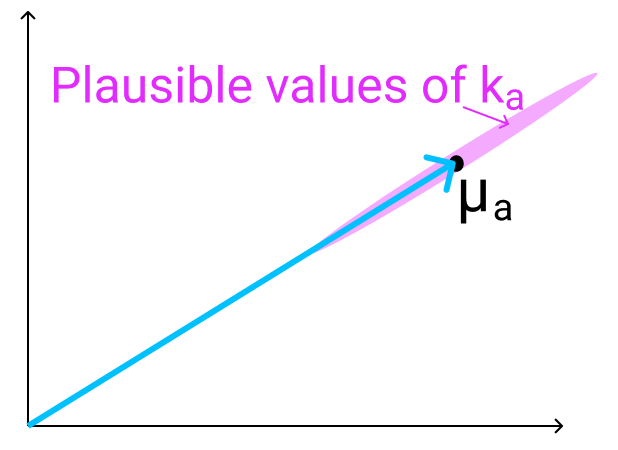
\includegraphics[width=0.35\linewidth]{images/ka_plausible.png}
\caption{The vector $\mu_a$ (shown here in 2D as an example), with the range of possible values of $k_a$ shown in red. As mentioned previously, $k_a$ points in roughly the same direction as $\mu_a$, but may have larger or smaller magnitude.}
\label{ka_plausible}
\end{figure}

When you sample $\{k_1,\dots,k_n\}$ multiple times, and use the $q$ vector that you defined in part i., what do you expect the vector $c$ will look like qualitatively for different samples? Think about how it differs from part (i) and how $c$'s variance would be affected.

\ifans{
    According to the previous questions, $q=\lambda(\mu_a+\mu_b)$, where $\lambda \gg 0$, which mean $q$ is a linear combination of $k_a$ and $k_b$ and orthogonal to $k_i$, where $i \in \{1, 2, \ldots, n\}, i\neq a, i\neq b$.
    
    \begin{equation}
        \begin{aligned}
            k_a &\approx \epsilon \mu_a \\
            k_i &\approx \mu_i, i \neq a \\
        \end{aligned}
    \end{equation}

    \begin{equation}
        \begin{aligned}
            k_a^Tq &\approx \epsilon \mu_a^T \lambda(\mu_a+\mu_b) = \epsilon\lambda \\
            k_b^Tq &\approx \mu_b^T \lambda(\mu_a+\mu_b) = \lambda \\
            k_i^Tq &\approx \mu_i^T \lambda(\mu_a+\mu_b) = 0, i \neq a, i \neq b \\
        \end{aligned}
    \end{equation}

    \begin{enumerate}
        \item When $epsilon > 1$, $k_a^Tq > k_b^Tq$, which means $c \approx v_a$.
        \item When $epsilon = 1$, $k_a^Tq = k_b^Tq$, which means $c \approx \frac{1}{2}(v_a + v_b)$.
        \item When $epsilon < 1$, $k_a^Tq < k_b^Tq$, which means $c \approx v_b$.
    \end{enumerate}

    Therefore, $c$ will oscillate between $v_a$ and $v_b$ when $epsilon$ changes, which means $c$'s variance will be affected.
}
\end{subparts}

\part[3] \textbf{Benefits of multi-headed attention:}
Now we'll see some of the power of multi-headed attention.
We'll consider a simple version of multi-headed attention which is identical to single-headed self-attention as we've presented it in this homework, except two query vectors ($q_1$ and $q_2$) are defined, which leads to a pair of vectors ($c_1$ and $c_2$), each the output of single-headed attention given its respective query vector.
The final output of the multi-headed attention is their average, $\frac{1}{2}(c_1+c_2)$.
As in question 1(\ref{q_problem_with_single_head}), consider a set of key vectors $\{k_1,\dots,k_n\}$ that are randomly sampled, $k_i\sim \mathcal{N}(\mu_i, \Sigma_i)$, where the means $\mu_i$ are known to you, but the covariances $\Sigma_i$ are unknown.
Also as before, assume that the means $\mu_i$ are mutually orthogonal; $\mu_i^\top \mu_j = 0$ if $i\not=j$, and unit norm, $\|\mu_i\|=1$.
\begin{subparts}
\subpart[1]
Assume that the covariance matrices are $\Sigma_i=\alpha I$, for vanishingly small $\alpha$.
Design $q_1$ and $q_2$ such that $c$ is approximately equal to $\frac{1}{2}(v_a+v_b)$. 
Note that $q_1$ and $q_2$ should have different expressions.

\ifans{
    Multi-head attention is more flexiable than single-head attention. We can get more $q_1$ and $q_2$ combinations such that $k_a^Tq_1=k_b^Tq_2$, which indicates $c$ is approximately equal to $\frac{1}{2}(v_a+v_b)$. For example:
    
    \begin{equation}
        q_1 =q_2= \lambda(\mu_a+\mu_b)
    \end{equation}

    \begin{equation}
        \begin{aligned}
            q_1 &= \lambda\mu_a \\
            q_2 &= \lambda\mu_b \\
        \end{aligned}
    \end{equation}

    where $\lambda \gg 0$.
}

\subpart[2]
Assume that the covariance matrices are $\Sigma_a=\alpha I + \frac{1}{2}(\mu_a\mu_a^\top)$ for vanishingly small $\alpha$, and $\Sigma_i=\alpha I$  for all $i \neq a$.
Take the query vectors $q_1$ and $q_2$ that you designed in part i.
What, qualitatively, do you expect the output $c$ to look like across different samples of the key vectors? Explain briefly in terms of variance in $c_1$ and $c2$. You can ignore cases in which $k_a^\top q_i < 0$. 

\ifans{
    \begin{itemize}
        \item If $q_1 =q_2= \lambda(\mu_a+\mu_b)$, different heads will behave like single-head attention, which means $c$ will oscillate between $v_a$ and $v_b$ when $epsilon$ changes, which means $c$'s variance will be affected.
        \item If $q_1 = \lambda\mu_a$ and $q_2 = \lambda\mu_b$, $c$ will be a linear combination of $v_a$ and $v_b$, which means $c$'s variance will not be affected. Different head will focus on different elements in the sequence at the same time.
    \end{itemize}
}



\end{subparts}







\end{parts}